\section{Probability}
This section gives an introduction to some tools and ideas from probability theory. One of the main reasons for including it is that it lets us give background to the final sub-section on Brownian motion, but we'll also use some of the methods from here in the final section of the course on complex networks.

Physical variables can be either continuous or discrete. Continuous variables, like the spatial position of a particle ${\bf r} = (x,y,z);$ $x\rightarrow x+dx$ allow us to apply tools from differential calculus. Discrete variables (like the spin of an electron, the face of a playing card, or the energy level of a quantum particle) require a different approach. As the number of discrete states gets gets large, it is possible to approximate a discrete system by a continuous one. However, there are often statistical reasons why this is not always the best approach. (For one example of why it is not always good to approximate a discrete distribution with a continuous one, see the article ``Power-Law Distributions in Empirical Data'' \cite{powerlawdist})

Here we are going to look at some simple discrete distributions, including one of the simplest --- the binomial distribution which describes the probability of events that can take one of only two possible outcomes. The tool we will employ to study these distributions is \emph{probability generating functions} (PGFs) (or generating functions for short). Although PGFs can be somewhat cumbersome, they provide a powerful general tool that can applied to a wide range of situations involving discrete probabilities. In this sense they are like the Taylor series of discrete probability.

\subsection{Probability generating functions}
\begin{definition}[Probability Generation Function / PGF]
We call a polynomial $\calG:\mathbb{R}\mapsto\mathbb{R}$ a Probability Generating Function if

$$\calG(x) = \sum_{n=0}^\infty P(X=r_n)x^n$$

where $P(X=r_n)$ is the probability that $X=r_n$.
\end{definition}

For example, the PGF for an equal probability die is 
$$\calG(x) = 0x^0+\frac16x^1+\frac16x^2+\frac16x^3+\frac16x^4+\frac16x^5+\frac16x^6.$$
As an example of how PGFs are a handy general tool, say we now wanted to find the PGF for the sum when we roll two such dice. We can just multiply the PGFs to get $\calG'(x) = \calG(x)\calG(x) = 0x^0 + 0x^1+\frac{1}{36}x^1x^1+\frac{2}{36}x^1x^2+\cdots+\frac{1}{36}x^6x^6.$

More generally, the set of probabilities associated with any discrete distribution can be used as coefficients of $\calG(x)$:
$$\calG(x) = P(X=r_0)x^0+P(X=r_1)x^1+\cdots = \sum_{n=0}^\infty P(X=r_n)x^n.$$

\subsection{Properties of generating functions}
\begin{eqnarray*}
	\calG(0)&=&P(X=0)\\
	\calG(1)&=&\text{sum over all probabilities}=1
\end{eqnarray*}
The two properties above are easy to see and are not unexpected. More interesting is the fact that derivatives of PGFs can be used to obtain expressions for the mean, and higher order moments, of the distribution associated with the PGF.

\begin{eqnarray*}
	\frac{d}{dx}\calG(x)=\calG'(x)&=&\sum_r rP_r x^{r-1},\qquad\text{and}\\
	\calG''(x)&=&\sum_r r(r-1)P_rx^{r-2}.
\end{eqnarray*}

If we evaluate the first derivative of the PGF at 1 we get
$$\calG'(1) = \sum_r rP_r.$$
The expected value of an arbitrary function $f(r)$ is given by $\langle f(r)\rangle = \sum_r f(r) P(X=r)$, therefore $\calG'(1) = \langle r\rangle$ --- the expected value, or mean, of the distribution.

Similarly,  Evaluating $\calG''(x)$ at 1 gives 
$$\calG''(1) = \sum_r r(r-1)P(X=r) = \langle X(X-1)\rangle.$$

Why would we care about being able to find $\langle X(X-1)\rangle = \langle X^2 -X\rangle$? Because the variance of X, is given by 
$$ V(X) = \langle X^2\rangle -\langle X\rangle^2.$$ We are therefore able to construct $V(X)$ from combinations of $\calG$, $\calG'$, and $\calG''$.
We can use the fact that $\langle X^2 -X\rangle =\langle X^2\rangle-\langle X\rangle$ I.e. $\sum(r^2-r)P(X=r)=\sum r^2P(X=r)-\sum rP(X=r)$ to get

\begin{eqnarray}
V(X)&=&\langle X^2\rangle - \langle X\rangle^2\\
&=&\underbrace{\langle X^2\rangle -  \langle X \rangle}_{\calG''(1)} + \underbrace{\langle X\rangle}_{\calG'(1)} - \underbrace{\langle X \rangle^2}_{\calG'(1)^2}\\
&=& \calG''(1) +\calG'(1)-\calG'(1)^2 \label{eq:binvar}
\end{eqnarray}

%Generating functions may not always be the shortest way to find the properties of some distribution, but they are a powerful way.

\subsection{The binomial distribution}
The binomial distribution describes the probability of getting $r$ identical outcomes from a sequence of $N$ events where each event has only two possible states, e.g. number of heads from a sequence of coin tosses, number of Au atoms from deposition of Au and Ag atoms in some sputtering process, or number of spin up electrons in an uncorrelated system.

The probabilities for the binomial distribution are given by
$$P(X=r) = \binom{N}{r}p^rq^{N-r}, ~\text{ where } \binom{N}{r} = \frac{N!}{r!(N-r)!}, ~~r=0,1,\ldots,N$$
and where (mostly) $p+q=1$.
The PGF for the binomial distribution is therefore given by $\calG(x) = \sum_{r=0}^N\binom{N}{r}p^rq^{N-r}x^r$. 
The coefficients in the binomial distribution are (not surprisingly) the coefficients from the  binomial expansion theorem. This means that instead of writing the PGF as a sum, we can easily express it (and its derivatives) as a polynomial:
\begin{eqnarray*}
	\calG(x)  &=& (xp +q)^N \\
	\calG'(x) &=& N(xp+q)^{N-1}p\\
	\calG''(x) &=& N(N-1)(xp+q)^{N-2}p^2. 
\end{eqnarray*}

Evaluating the above at $x=1$ gives:
	\begin{eqnarray*}
	\calG(1) &=& (p+x)^N = 1 ~\text{ if } p+q=\\
	\calG'(1) &=& N(p+q)^{N-1}P = Np  ~\text{ if } p+q=1\\
	\calG''(1) &=& N(N-1)(p+q)^{N-2}p^2 \\
		&=&N(N-1)p^2  ~\text{ if } p+q=1.
\end{eqnarray*}
As expected, we have $\langle X\rangle =Np$ for the event associated with the probability $p$.
Similarly, we can calculate the variance of the binomial distribution using equation \ref{eq:binvar}
\begin{eqnarray*}
	V(X) &=&\calG''(1) - \calG'(1) -\calG'(1)^2\\
		&=& N^2p^2-Np^2+Np-N^2p^2\\
		&=& N(p-p^2)\\
		&=& Np(1-p)= Npq.
\end{eqnarray*}

If you are feeling enthusiastic, compare the calculation above with the usual method for finding the variation of the binomial distribution without using a PGF.

\subsection{The expected long-run outcome of a binary process}
What is the net outcome we can expect from a sequence of $N$ binary events? What is the variance in this net outcome? How long can we expect the net outcome to remain positive? 

Think of a sequence of coin tosses where heads implies $+1$ and tails implies $-1$. We will denote the number of heads from $N$ events as $n_h$ and the number of tails as $n_t = N-n_h$, then the net outcome is $d = n_t-n_h = N-2n_h$. 

If $p=q=\frac12$ then the expected value of $d$ is $\langle d\rangle= 0$. (It's easy to check this: $\langle d\rangle = \langle N-2n\rangle = N-2\langle n\rangle = N-\frac{2}{2}N=0.$)

We want to find the variation in $d$, or rather, the root-mean-squared (rms) deviation 
$$d_{rms} = \left(\langle d^2\rangle - \langle d\rangle^2\right)^{\frac12} =  \langle d^2\rangle^{\frac12}.$$

At this point we'll drop the subscript in $n$ since we only have $n_h$ and since the probabilities are equal. From $d=N-2n$ we have $$ \langle d^2\rangle = \langle (N-2n)^2\rangle = \langle N^2 -4Nn+4n^2\rangle.$$
We know that $\langle n\rangle = \calG'(1)=Np=N/2$ and from the expressions for $\calG''(1)$ and $\calG'(1)$ we get $\langle n^2 \rangle = \calG''(1) + \calG'(1)$ where $\calG''(1) = N^2p^2 = N^2/4-N/4$. We can now calculate $\langle d^2 \rangle$.

\begin{eqnarray*}
	\langle d^2 \rangle &=& N^2 -4N\frac{N}{2}+4\left(\frac{N^2}{4}-\frac{N}{4}+\frac{N}{2}\right)\\
		&=& N^2-2N^2+N^2+N\\
		&=& N.
\end{eqnarray*}
So, $d_{rms}=\sqrt{N}$ and the variance in the net expected outcome scales like $\sqrt{N}$ as $N$ increases. I.e. after $N$ steps we expect to be a rms distance of $\pm \sqrt{N}$ away from the mean of zero.

We can now look at how this would change if the binary process had some small bias $\alpha = |p-q| >0$. In this case, at each step, the expected outcome is $\alpha$ and the bounds for the rms distance from the mean are $\alpha N\pm\sqrt{N}$. See Fig.~\vref{fig:cointoss} for an example.

\begin{figure}[h]
    \centering
    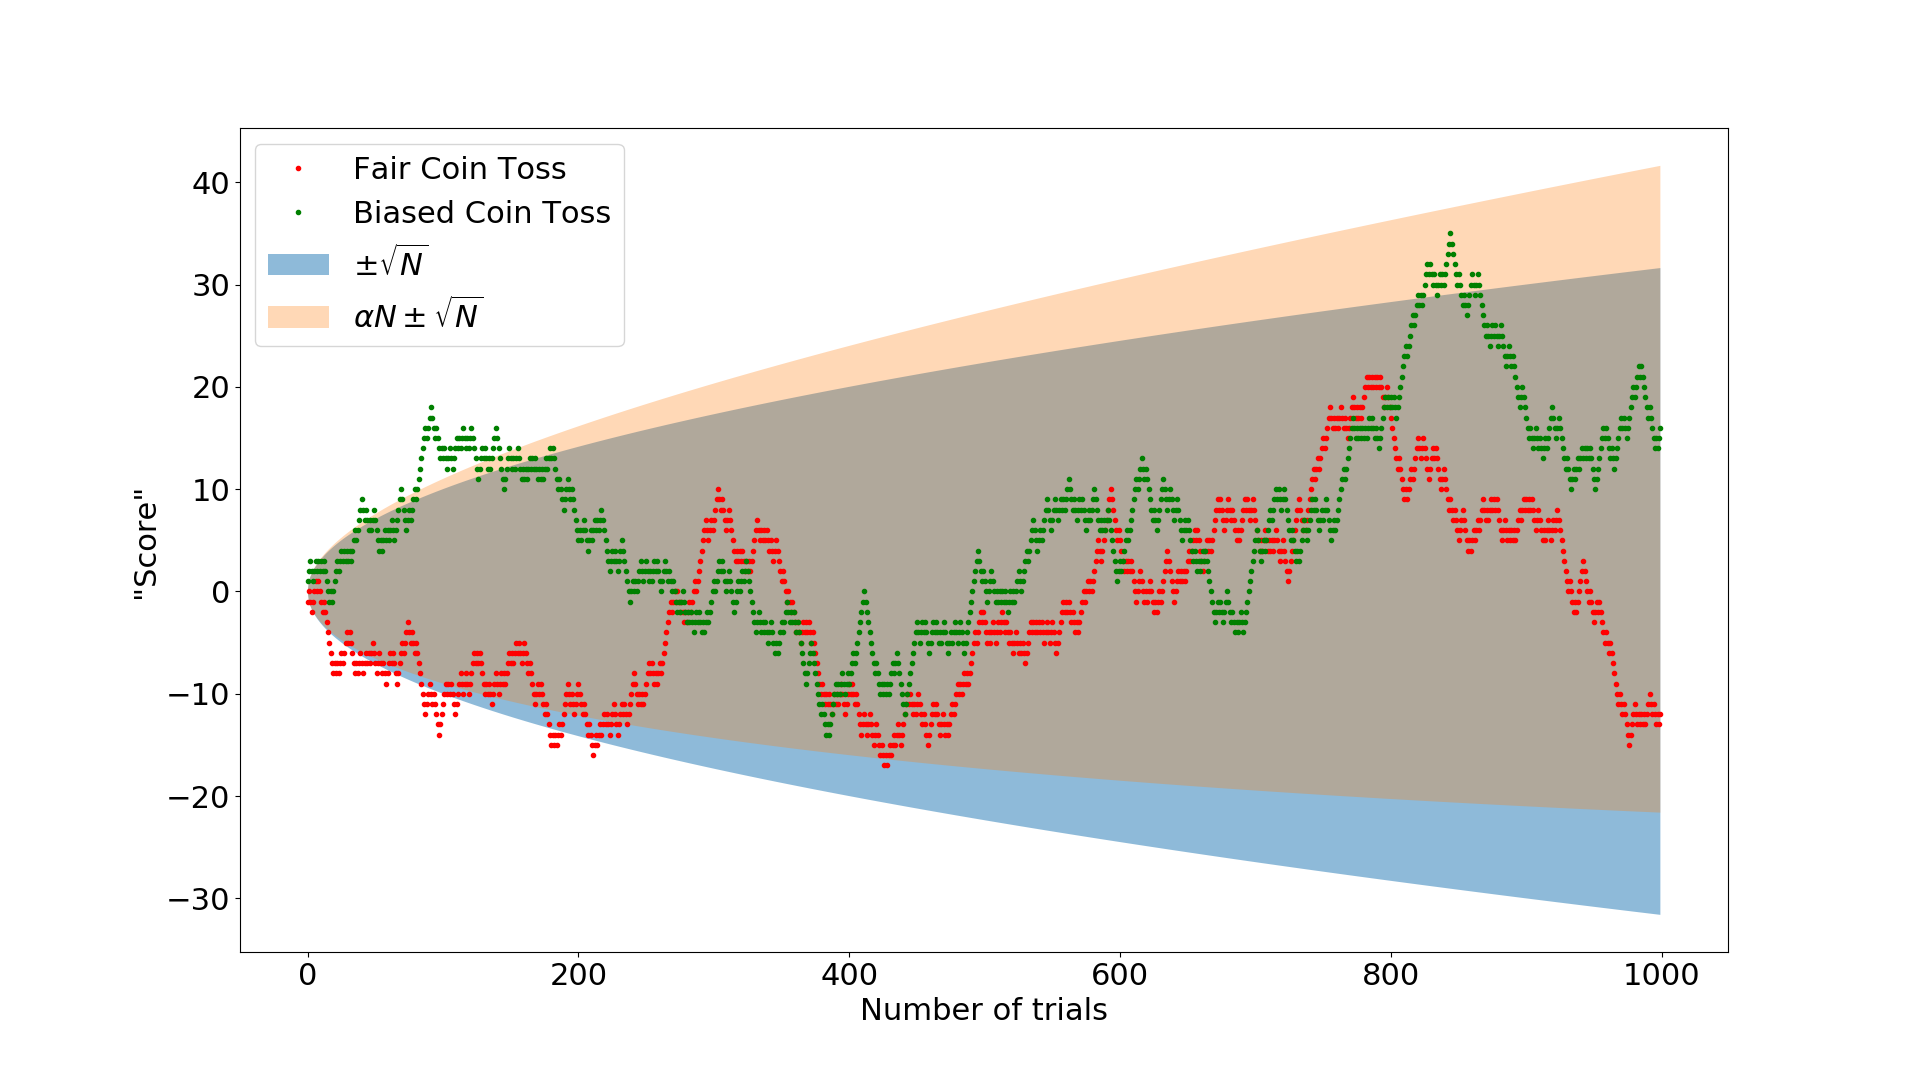
\includegraphics[width=\textwidth]{CoinToss}
    \caption{Long-run probability for a coin toss ($\alpha=0.01$). The shaded regions indicate the region between the rms distances.}
    \label{fig:cointoss}
\end{figure}

\subsection{Brownian motion}
Brownian motion is a model that describes the behaviour of particles in suspension (e.g. of dust in air, fine silt in dirty water) that have some velocity but which are constantly changing direction as they are buffeted by other particles. Their motion can be understood through a calculation similar to that for the net outcome of the binary process above, but in 3D.

The conceptual model that is often used when discussing Brownian motion is that of a \emph{random walk}. Consider a random walker who after $n$ steps is at the position ${\bf r} = (x,y,z)$. Each step is given by ${\bf s}_{n+1} = {\bf r}_{n+1}- {\bf r}_n$ and has step length $s_n$ in a random and uncorrelated direction ${\bf\hat{s}}_n$. Again (by symmetry) $\langle {\bf s}\rangle =0$. We want to find how far a particle might have gone after $N$ steps. We will define $\lambda^2= \langle {\bf s}^2\rangle$ --- the average square step-length. We write ${\bf r}_N$ for the position of the walker (or the particle) after $N$ steps, then
\begin{eqnarray*}
	\langle {\bf r}_N^2 \rangle &=& \bigg\langle \left(\sum_{n=1}^N{\bf s}_n\right)^2 \bigg\rangle\\
		&=& \bigg\langle \sum_{n=1}^N{\bf s}_n^2 +2\sum_{n=1}^{N-1}\sum_{m=n+1}^N{\bf s}_n\cdot{\bf s}_m \bigg\rangle\\
		&=& \sum\underbrace{\langle {\bf s}_n\rangle}_{=\lambda^2} + 2\sum\sum \underbrace{\langle {\bf s}_n \cdot {\bf s}_m \rangle}_{=\langle {\bf s}_n\rangle \cdot \langle{\bf s}_m \rangle=0}
\end{eqnarray*}

The first term in the expression is the mean squared step-length while the second term is zero since there is no correlation between the directions of each of the steps. Hence $\langle {\bf r}_N\rangle = N\lambda^2$ and the rms displacement is $\sqrt{N}\lambda$. If the number of steps is proportionate to the length of time that the particles move for, then we have that the mean-square displacement scales like $\sqrt{t}$. This is one of the key features of diffusive processes. 




